\Chapter{Megvalósítás}

\Section{Adatok előkészítése}
Az előző fejezetben leírtam, hogy mi az a 4 lépés ami ahhoz kell, hogy egy pontos modellt tudjunk építeni. Az 1. lépés az adatok összegyűjtése volt. Számomra az adatgyűjtést nem kellett elvégezni hiszen rendelkezésre állt az adathalmaz, így mehetünk is a második lépésre, ami az adatok előkészítése.

\subsection{Üres érték vizsgálata}
\begin{python}
data.isnull().any()
\end{python}
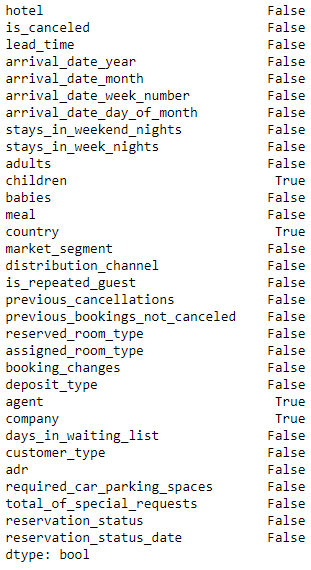
\includegraphics[scale=0.7]{images/4.fejezet/1.adatelokeszites.PNG}

Ez alapján látom a 4 változót, aminek oszlopaiban található üres érték. A 4 változó a következő: \texttt{children, country, agent, company}. Nézzük meg, hány százalékában található az oszlopokban.

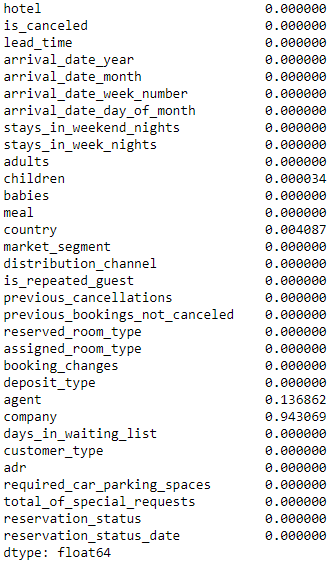
\includegraphics[scale=0.7]{images/4.fejezet/1.adatelokeszites1.PNG}

A \texttt{children} változónak 0.0034\%, a \texttt{country} változónak 0.4087\% , az \texttt{agent} változónak 13.68\%, a \texttt{company} változónak pedig 94.30\% értéke hiányzik.

Ezekkel a következő teendők lehetnek:
\begin{itemize}
    \item Ezeket az oszlopokat amikben hiányzó érték van egyszerűen törlöm.
    \item Behelyettesítek az átlagos/medián/módusz értékével az adott oszlopnak.
    \item Nem csinálok vele semmit, és hagyom úgy ahogy vannak.
\end{itemize}

Azonban ezek közül a megoldások nem lehet egyértelműen választani, hogy melyik adatkészlethez melyik jó anélkül, hogy megvizsgálnám ezeket az oszlopokat és elgondolkozzok, hogy ahol hiányzik érték milyen okból kifolyólag hiányozhat.

Például, ha egy olyan adatkészletem van ami, házaknak az árát becsüli meg abból, hogy melyik szoba mekkora, hány szoba van, van-e garázs és hiányzik néhány sorban arról adat, hogy mekkora a nappali akkor rossz döntés az, hogy az egész oszlopot töröljük, hiszen ez esetben rengeteg értékes adatot szedünk ki amivel a jövőben a modellem pontossága csökkenhet. Egy ilyen esetben mivel általában minden háznak van nappalija elképzelhető, hogy az adatok elvesztek út közben, ezért célszerű lehet a hiányzó adatokat az oszlop átlagával/mediánjával/móduszával behelyettesíteni. Ha azonban az adatoknak kevesebb mint 1\%-nál nem található csak, hogy mekkora a nappali méret, feltételezhetjük, hogy ezeknek a házaknak valóban nincs nappalijuk, és a legcélszerűbb ilyenkor úgy hagyni ahogy vannak.

\subsubsection{\texttt{children} oszlop vizsgálata}
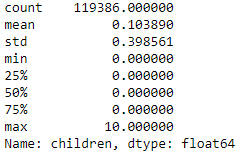
\includegraphics{images/4.fejezet/2.adattisztitas.PNG}

A gyerekek számának átlaga 0.1 és ha a gyerek számát növekvő sorrendbe rendezve is láthatom, hogy az első 75\%-ban 0 gyerekkel foglaltak szállást. Így a \texttt{children} oszlop hiányzó értékeit behelyettesíthetem 0-val, ugyanis elég valószínű, hogyha ez az adat hiányzik akkor a szállást foglalok nem vittek gyereket, valamint ha átlag, medián vagy módusz alapján helyetesítenék be ezt az értéket akkor is 0-val kellene.

\subsubsection{\texttt{country} oszlop vizsgálata}
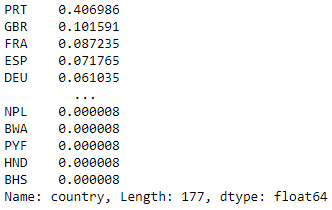
\includegraphics{images/4.fejezet/2.adattisztitas1.PNG}

Mint látható itt 177 különböző kategóriájú adat van. Azonban ennek a 72.86\%-át az első 5 leggyakrabban jelenlévő ország teszi ki. Így a hiányzó értékek mellett rengeteg olyan értékem is va, ami maximum egyszer-kétszer jelenik meg az adathalmazban. Ezek az értékek sokkal nem segítik a modell pontosságát, hiszen maximum egy-kettő olyan sort fognak látni, amit egy adott országból foglaltak. Így gondolhatnám azt is, hogy mivel a 177 különböző országból 5 teszi ki a foglalások nagy részét, hogy ezt az oszlopot csak simán el lehet hagyni, hiszen az országok többségéről nem fog sok mindent megtudni a modell abból a pár sorból amiben egy adott nemzet szerepel. Én viszont azt a lehetőséget választanám, hogy az első 5 országot úgy hagyom ahogy vannak, a többit és ahol hiányzó értékek vannak pedig egy "other" értékre cserélném, így a modellem nem fog olyan országot látni, ami csak pár sorban szerepel. A hiányzó értékeket azért lehet biztonságosan other-re cserélni, ugyanis egy adott vendégnek a világ valamelyik országából mindenféleképpen érkeznie kell.

Az új country oszlop  így néz ki a csere után.

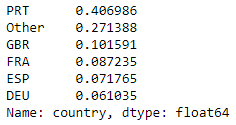
\includegraphics{images/4.fejezet/2.adattisztitas2.PNG}

\subsubsection{\texttt{agent} és \texttt{company} oszlopok vizsgálata}

Ez a két oszlop vélemény szerint közel áll egymáshoz, ezért lehet a két oszlopot egyszerre vizsgálni azzal kapcsolatban, hogy mit csináljak a null értékekkel.
\begin{itemize}
    \item \texttt{agent}: Ez annak az utazási irodának az id-jét tartalmazza amelyik a foglalta a szállást. Így, ha ez az érték null akkor valószínűleg nem utazási irodán keresztül lett foglalva a szállás.
    \item \texttt{company}: Ez annak a cégnek az id-jét tartalmazza, amelyik foglalta a szállást vagy felelős a fizetésért. Így, ha ez az érték null feltétlezhetem a foglalás privát úton történt és nem volt szükség egy ilyen közbenjáróra.
\end{itemize}
Így null értéket egy "None" értékkel fogom helyetesíteni.

\subsection{Rendellenes érték vizsgálata}

\subsubsection{\texttt{adr} oszlop vizsgálata}
Miközben nézegettem a különböző statisztikákat az adatokról, ennél a változónál észrevettem egy furcsa dolgot, ami a következő.

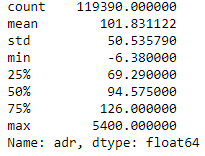
\includegraphics{images/4.fejezet/2.adattisztitas3.PNG}

A legkisebb érték -6.38 ami azt jelenti, hogy a szállás fizetett a vendégnek azért, hogy ott tartozkódjon. Azért nem igazán szokott előfordulni, úgyhogy megvizsgáltam hány 0-nál kisebb adr értékkel rendelkező sor található az adathalmazban és ezeket a sorokat kiírattam.

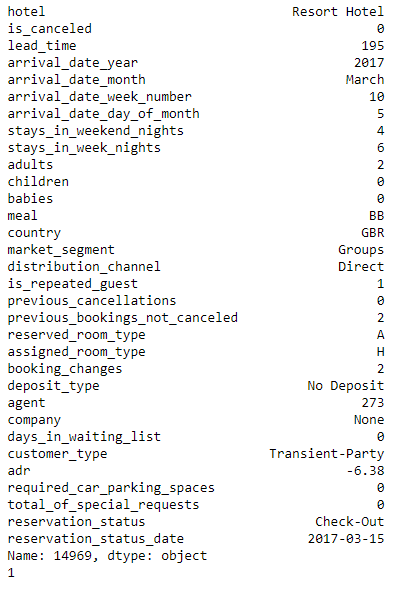
\includegraphics[scale=0.55]{images/4.fejezet/2.adattisztitas4.PNG}

Csupán egy érték van ami kisebb 0-nál. Semmi különöset nem veszek észre ebben a sor adatban. A foglalást nem mondták le, a reservation\_status: Check-out amit az ott tartózkodásuk végén módosítottak tehát nem mentek el hamarabb a szállodából akármilyen okból. Így úgy gondoltam, hogy ez az egy érték is rendben legyen behelyetesítettem ennél a sornál az adr-t az átlagos adr értékével.

\Section{Adatelemzés}

Ez a lépés azért szükséges, hogy jobban megértsem az adathalmazt, a különböző változók között álló kapcsolatokat, melyek a fontosabb változók a modell szempontjából. Az előző lépésnél foglalkoztam a szembetűnőbb hibákkal, azonban ennél a résznél is előfordulhatnak még anomáliák az adatokkal.

Ez a lépés azzal kezdődik, hogy feltevéseket vetettem fel az adathalmazzal kapcsolatban, majd ezekre kerestem igazolást vagy cáfolatot.

\subsection{Kapcsolat a foglalás és érkezés idejével}

\textit{Minél hamarabb foglalják le a szállást az érkezés dátumához képest annál nagyobb valószínűséggel mondják le.}
Csináltam egy pivot táblát amiben a következő változókat raktam bele: \texttt{is\_canceled} és \texttt{lead\_time}

\begin{center}
\begin{tabular}{ c c  }
  & lead\_time \\ 
 is\_canceled &  \\  
  0 & 79.984687 \\
  1 & 144.848815
\end{tabular}
\end{center}

Ebből azt láthatom, hogy a feltevése, miszerint minél hamarabb foglalják le a szállást az érkezés dátumához képest annál nagyobb valószínűséggel mondják le igaz, hiszen a lemondott foglalásoknak (1) majdnem kétszer nagyobb a lead\_time-ja, mint a nem lemondottaknak.

Azonban meg szeretném nézni azt is, hogyan oszlik el külön-külön a lemondott és a nem lemondott foglalások lead\-time-ja. Erre a következő vonaldiagrammot hoztam létre.

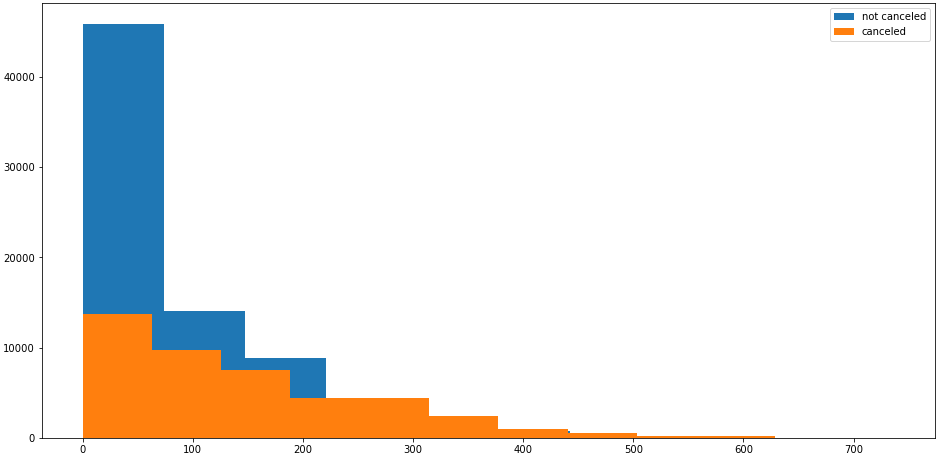
\includegraphics[scale=0.57]{images/4.fejezet/3.adatelemzes1.PNG}

Ebből azt látom, hogy a két diagram az elején, azaz a kis lead\_time-oknál különöl el a legjobban, minél nagyobb annál jobban egybeolvad. Ezek szerint a nem lemondott foglalások nagyrésze néhány nappal az érkezés dátuma előtt történt.

Így a fenti feltevés nem igazán állja meg a helyét, és javítanám arra, hogy minél közelebb foglalták le a szállást az érkezés dátumához képest annál nagyobb valószínűséggel érkezik meg a vendég.

\subsection{Hétköznapi és hétvégi lemondások arányai}

\textit{Hétvégén kevesebb foglalást mondanak le, mint hétköznap.}
\begin{python}
only_week_night = data.loc[data["stays_in_weekend_nights"] == 0,
"stays_in_week_nights"].count()
only_weekend_night = data.loc[data["stays_in_week_nights"] == 0,
"stays_in_weekend_nights"].count()
only_week_night_no_cancel=data.loc[(data["stays_in_weekend_nights"]==0)
&(data["is_canceled"] == 0), "stays_in_week_nights"].count()
only_weekend_night_no_cancel=data.loc[(data["stays_in_week_nights"]==0)
&(data["is_canceled"] == 0), "stays_in_weekend_nights"].count()
print("Csak hetkoznap: {: .2f} lemondva"
.format(1-(only_week_night_no_cancel/only_week_night)))
print("Csak hetvege: {: .2f} lemondva"
.format(1-(only_weekend_night_no_cancel/only_weekend_night)))
\end{python}
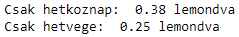
\includegraphics{images/4.fejezet/3.adatelemzes2.PNG}

13\%-kal kevesebb foglalást mondanak le a hétvégéken. Valószínűleg azért, mert az embereknek a hétköznapokban munka vagy akármilyen más ügyei lehetnek, amik miatt le kell mondani a foglalást. Akár egyik napról a másikra is. Ez gondot jelent a szállodáknak, ugyanis minél később mondja le a foglalását egy vendég, annál kevesebb ideje van eladni újra a szobát.

\subsection{Hétköznapi lemondások}

\textit{Hétköznapokra történő foglalásokat gyakran mondják le 1-2 nappal érkezés előtt.}
\begin{python}
canceled_info=data[data["reservation_status"]=="Canceled"]
canceled_info_week_night=
canceled_info[canceled_info["stays_in_weekend_nights"]==0]
less_than_2_count = 0
for index, row in canceled_info_week_night.iterrows():
    arrival_year = row["arrival_date_year"]
    arrival_month = months[row["arrival_date_month"]]
    arrival_day = row["arrival_date_day_of_month"]
    status_change = row["reservation_status_date"].split("-")
    arrival_date = date(arrival_year, arrival_month, arrival_day)
    change_date = date(int(status_change[0]), int(status_change[1]),
    int(status_change[2]))
    if (arrival_date-change_date).days < 3:
        less_than_2_count+=1
print("A foglalasok{: .2f}van legfeljebb 2 nappal erkezes elott lemondva"
.format(less_than_2_count/len(canceled_info_week_night)))
\end{python}
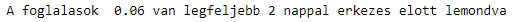
\includegraphics{images/4.fejezet/3.adatelemzes3.PNG}

Csupán a foglalások 6\%-a van legfeljebb 2 nappal érkezés előtt lemondva.  Ezáltal az ezekben a szállodákban foglalt vendégeknek csupán töredékének kellett 1-2 nappal érkezés előtt lemondania a szállást. Így hibás volt a feltevés, hogy hétköznaponta sok foglalásokat gyakran mondják le 1-2 nappal érkezés előtt.

\subsection{Felnőttek hatása}
\textit{Minél több felnőtt van a foglalásban annál nagyobb valószínűséggel mondják le.}

Ezt a feltevést azért tartom valószínűnek, hiszen minél több felnőtt foglal le egy szállást annál több azoknak a személyeknek a száma akik miatt lehet le kell mondani, hiszen bármikor közbe jöhet valakinek valami.
\begin{python}
print("Atlagos felnottek szama az osszes foglalas figyelembe 
vetelenel:{:.4f}".format(data["adults"].mean()))
\end{python}

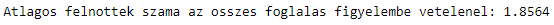
\includegraphics{images/4.fejezet/3.adatelemzes4.PNG}

\begin{center}
\begin{tabular}{ c c  }
  & adults \\ 
 is\_canceled &  \\  
  0 & 1.829737 \\
  1 & 1.901728
\end{tabular}
\end{center}

A lemondott foglalásoknal a felnőttek számának átlaga minimálisan nagyobb azonban ez nem hiszem, hogy akkora eltérés lenne, hogyha sok felnőtt foglalja le a szállást akkor nagy valószínűséggel levonhatnánk azt a következtetést, hogy le lesz mondva.

\subsection{Gyerekek hatása}
\textit{Ha az emberek visznek magukkal gyereket nagyobb valószínűséggel mondják le a szállást.}
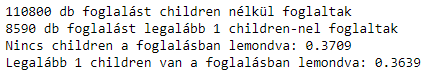
\includegraphics{images/4.fejezet/3.adatelemzes6.PNG}

A két eset között, hogy gyerekkel vagy gyerek nélkül mondják-e le nagyobb valószínűséggel a foglalást nincs nagy eltérés. Valamint a két különböző esetnek nagyban eltér a rendelkezésre álló adatmennyiség (egyik esetről 110800 példánk van a másikról csupán 8590), ezért az állítást, hogy akik gyerekkel foglaltak szállást nagyobb valószínűséggel mondják nem tudom magabiztosan igazolni.

\subsection{Babák hatása}
\textit{Ha babával utaznak az emberek akkor nagyobb valószínűséggel mondják le a foglalást.}

Mivel a babák még a gyerekeknél is kényesebb eseteket jelentenek ezért merem azt feltételezni, hogy nagyobb lesz a két eset között az eltérés mint a gyerekek esetében.

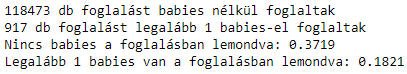
\includegraphics{images/4.fejezet/3.adatelemzes7.PNG}

Ebben a két esetben már elégnek mondható lenne az eltérés, hogy következtetéseket vonjak le. Azonban a rendelkezésre álló adatok arányával nagyobb baj van mint az előző vizsgálatnál, hiszen itt azoknak a foglalásoknak a száma amiben babával utaznak még az 1000 darabot sem éri el míg a másik esetben 118000-nél is több példánk van. Emiatt a hatalmas aránytalanság miatt ebből sem tudok biztos dolgot állítani.

\Section{Korrelációs mátrix és jelleg megállapítás}

Korrelációs mátrix azt mutatja meg hogy két vagy több változó mennyire függ egymástól. Tehát ha az egyik változik valamennyivel mennyivel fog változni a másik. Ez a mátrix fontos a jelleg megállapításhoz. Ugyanis a modellt elég lehet csak azokkal a változókkal tanítani amik a legjobban befolyásolják a kimenetelt. Ezzel is csökkentve a szükséges adatokat valamint a tanítási időt.
\subsection{Numerikus változók}

\begin{python}
plt.figure(figsize=(18,6))
sns.heatmap(data.corr().abs(), annot=True)
plt.show()
\end{python}

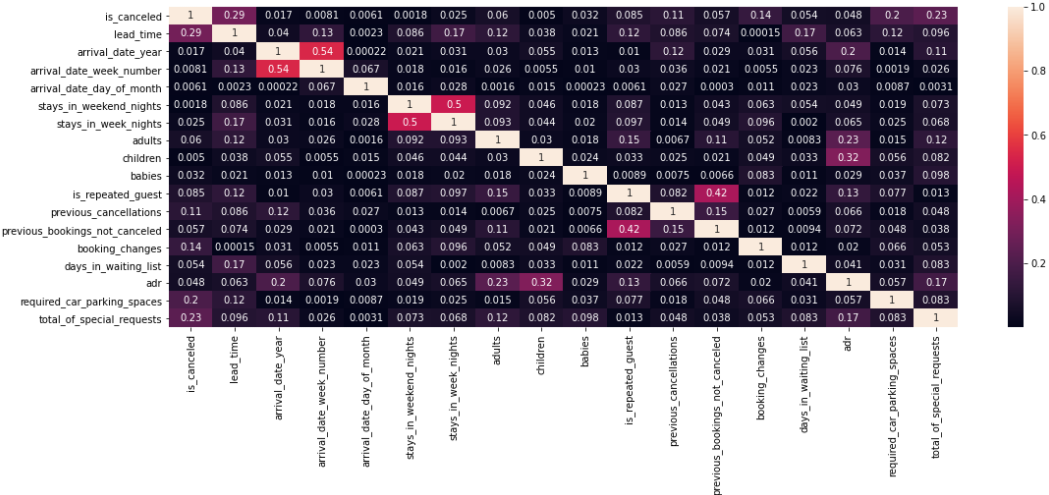
\includegraphics[scale=0.53]{images/4.fejezet/4.korrelacios.PNG}

Ezt a korrelációs mátrixot a következő képpen kell értelmezni. A korrelációs együttható minél közelebb van 1-hez annál jobban befolyásolja a két változó egymást és minél közelebb 0-hoz annál kevésbé. 
Ez alapján meg tudjuk állapítani, hogy az 5 legfontosabb numerikus változó:
\begin{enumerate}
    \item \texttt{lead\_time}
    \item \texttt{total\_of\_special\_requests}
    \item \texttt{required\_car\_parking\_spaces}
    \item \texttt{booking\_changes}
    \item \texttt{previous\_cancellations}
\end{enumerate}

Ezeket a változókat mindenféleképpen érdemes használni majd a modell építésénél. Vannak azonban olyanok is amiket ki vennék, hogy ne rontsa a modell pontosságát. Ilyen változó az \texttt{arrival\_date\_year} ugyanis az évek nem fognak ismétlődni a jövőben, tehát a modell semmi információt nem tud kiszedni abból, hogy egy adott foglalásnál látja hogy 2016-ban történt ha már 2020-at írunk. A \texttt{booking\_changes}-t is ki lehetne venni hiszen ez a változó folyamatosan változhat a foglalás pillanatától kezdve, de én ezt inkább benne hagyom hiszen hogyha egy foglalásnál a vendég módosít valamit akkor a modell újra tudja kalkulálni, a lemondás valószínűségét. Valamint a \texttt{days\_in\_waiting\_list} is elhagyható hiszen a modellünket arra az esetre akarjuk tanítani ha már a vendég be is foglalta a szállást, azonban amíg váró listában van ez nem történik meg.

\subsection{Kategorikus változók}

\begin{python}
cat_var=data[['is_canceled', 'hotel', 'meal', 'market_segment',
       'distribution_channel','reserved_room_type','assigned_room_type',
       'deposit_type', 'agent', 'company', 'customer_type']]
\end{python}


A \texttt{reservation\_status} változót mindenféleképpen el kell hagyni hiszen ebből a bemenetből a model rögtön meg is mondhatja a kimenetet hiszen ebben van eltárolva a foglalás állapota, hogy Check-Out (megérkezett a vendég és elhagyta a szállást) vagy Canceled (lemondta a foglalást) és ha ezt a változót töröljük akkor a \texttt{reservation\_status\_date} is szükségtelen, ami azt mutatja, hogy foglalás állapota mikor változott.

\subsubsection{Dummy változók}
Mielőtt kitérek a kategorikus változók korrelációs mátrixára először is a dummy változókról kell írnom. Hiszen a korreláció egy matematikai fogalom amibe számokkal tud számolni. Emiatt szükség van a mi kategorikus változóink átalakítására egész szám változókká. Ennek többféle módja van.
\begin{itemize}
    \item Label Encoding: Ez a módszer minden egyes kategóriát egy egész számra cserél. Ezzel az lehet a baj, hogy mivel a kategóriákat abc sorrendben cseréli ki egész számokra 0-tól kezdve, ezért önkéntelenül felállít egy számtani sorrendet a változók között. Amiből a mi esetünkben hiheti például azt a modell, hogy a 
    reggeli < félpanzió < teljes ellátás, amikor ilyesmiféle összefüggés nincs is közöttük. A meal oszlop így nézz ki label encoding-al:
    \begin{tabular}{ c c  }
      & meal \\ 
     meal &  \\  
      reggeli & 0 \\
      félpanzió & 1 \\
      teljes ellátás & 2
    \end{tabular}
    \item Dummy variables: Ez a módszer a meglévő adatokhoz új oszlopokat ad a következő módon. Minden egyes kategóriának új oszlopot csinál. Az oszlop értékei 0-át és 1-et vehetnek fel. Általában az 1-es jelenti, hogy teljesül a feltétel a 0 pedig ha nem. A meal oszlop így nézz ki dummy változókkal:
    
        \begin{tabular}{ c c c c }
          & meal\_reggeli & meal\_félpaznió & meal\_teljes\_ellátás \\ 
         meal &  \\  
          reggeli & 0  & 1 & 0\\
          félpanzió & 1  & 0 & 0\\
          teljes ellátás & 0 & 0 & 1
        \end{tabular}
\end{itemize}

Emiatt én a dummy változókat választottam a kategorikus változók korrelációs mátrixának létrehozás közben.

\begin{python}
cat_corr = pd.get_dummies(cat_var)
cat_corr.corr().abs().sort_values(ascending=False,
    by="is_canceled").head(10)
\end{python}

A kategorikus változók korrelációs mátrixa pedig így nézz ki a 10 legjelentősebb dummy változóval.

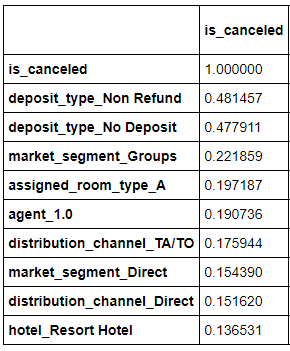
\includegraphics{images/4.fejezet/4.korrelacios1.PNG}

Ebből megállapítottam, hogy az 5 legfontosabb kategorikus változó a következő:
\begin{enumerate}
    \item \texttt{deposit\_type}
    \item \texttt{market\_segment}
    \item \texttt{assigned\_room\_type}
    \item \texttt{agent}
    \item \texttt{distribution\_channel}
\end{enumerate}

Megvizsgálom ezeket a változókat.
\subsubsection{\texttt{deposit\_type}}
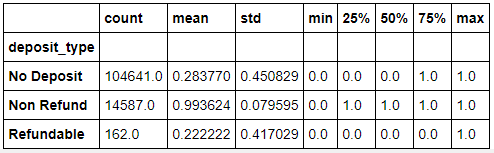
\includegraphics{images/4.fejezet/4.korrelacios2.PNG}

Mint láthatom a foglalások nagy többsége No Deposit-tal történt. Azonban ha jobban megvizsgálom az adatokat a Non Refund-nál észrevettem azt, hogy a lemondás átlaga nagyon magas 0.99 míg a másik két eset nem tér el nagyban egymástól. Ezt a változót jobban megvizsgálom ugyanis a kategorikus változóknál ez befolyásolja legjobban az \texttt{is\_canceled} változót így ha valami baj van vele az azt jelenti, hogy pontatalan lesz a modellem ha ezeket az adatokat is beleveszem.

\begin{python}
data.groupby("deposit_type").mean()
\end{python}
\scalebox{0.58}{
\begin{tabular}{llllll}
 & previous\_cancellations & is\_repeated\_guest & booking\_changes & required\_car\_parking\_spaces & total\_of\_special\_requests \\
deposit\_type &  &  &  &  &  \\
No Deposit & 0.042039 & 0.035760 & 0.249634 & 0.071129 & 0.651427 \\
Non Refund & 0.411462 & 0.004387 & 0.012477 & 0.000069 & 0.001782 \\
Refundable & 0.000000 & 0.024691 & 0.592593 & 0.123457 & 0.141975
\end{tabular}
}

A \texttt{previous\_cancellations}, a \texttt{is\_repeated\_guest}, a \texttt{booking\_changes}, a \texttt{required\_car\_parking\_spaces} és a \texttt{total\_of\_special\_requests} átlagjai nagyon eltérnek a Non Refund esetnél a másik kettőhöz képest. Ezek alapján az adatok alapján Non Refund-al olyan emberek foglaltak szállást akik az esetek majdnem felében mondtak már le foglalást, parkolóhelyre nincs szükségük, nagyon ritkán kérik hogy változtassanak valamit a foglalásban és kevés különleges kérésük van. Ezzel abban az esetben ha az \texttt{deposit\_type} (Előleg típusa) más lenne mint Non Refund (Nem visszatéríthető) nem lenne gond, viszont valószínűtlennek tartom, hogy az emberekek akik így foglalnak szállást hatalmas arányban mondják le, így hagyják veszni a pénzüket ezért inkább biztonságból kiveszem a \texttt{deposit\_type}-ot is a jelleg változók közül ugyanis ezek miatt lehetnek benne valótlan adatok.

\subsubsection{\texttt{market\_segment}}
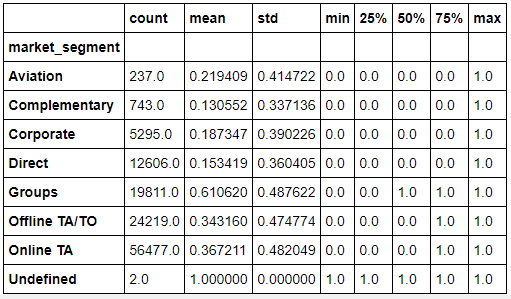
\includegraphics{images/4.fejezet/4.korrelacios3.png}

Ennél a változónál nem találtam az elérhető adatoknál különösebb rendelleneséget.

\subsubsection{\texttt{assigned\_room\_type}}
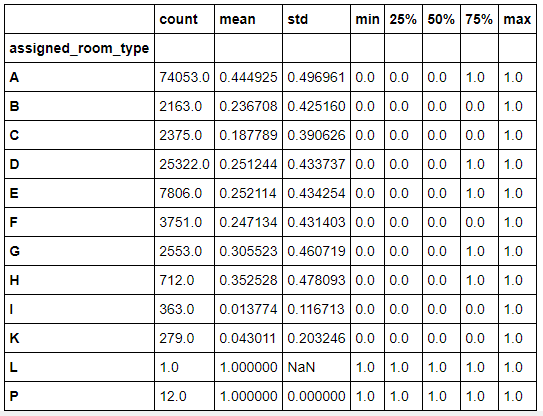
\includegraphics{images/4.fejezet/4.korrelacios4.png}

Ennél a változónál látható, hogy az L és P foglalt szobáknak 100\%-os a lemondási aránya, azoban L típusú szobából csupán 1 darabot foglaltak, P típusú szobából pedig 12 darabot. Ez töredéke az összes adatnak, így inkább benne hagyom ezt a változót mert úgy gondolom, hogy inkább javítani fog a modellem pontosságán mintsem rontani.

\subsubsection{\texttt{agent}}
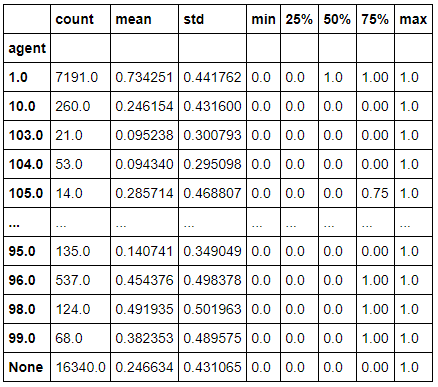
\includegraphics{images/4.fejezet/4.korrelacios5.PNG}

Ennél a változónál nem találtam az elérhető adatoknál különösebb rendelleneséget.

\subsubsection{\texttt{distribution\_channel}}
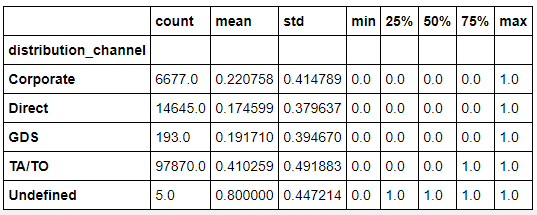
\includegraphics{images/4.fejezet/4.korrelacios6.PNG}

Ennél a változónál nem találtam az elérhető adatoknál különösebb rendelleneséget.